\documentclass[12pt,twoside, a4paper, twocolumn]{article}
\usepackage[utf8]{inputenc}
\usepackage[brazil]{babel}
\usepackage[margin = 0.5in]{geometry}
\usepackage{amsmath}
\usepackage{amsthm}
\usepackage{amssymb}
\usepackage{amsthm}
\usepackage{setspace}
\usepackage[americanvoltages,fulldiodes,siunitx]{circuitikz}
\usepackage{lipsum}
\usepackage{pgfplots}
\usepackage{ifthen}
\usepackage{adjustbox}
\usepackage[section]{placeins}
\usepackage{hyperref}
\usepackage{graphicx}
\usepackage{amsmath}
\usepackage{amsthm}
\usepackage{amssymb}
\usepackage{amsthm}
\usepackage{setspace}
\usepackage[americanvoltages,fulldiodes,siunitx]{circuitikz}
\usepackage{lipsum}
\usepackage{pgfplots}
\usepackage{ifthen}
\usepackage{adjustbox}
\usepackage[section]{placeins}
\usepackage{hyperref}
\usepackage{graphicx}
\usepackage{adjustbox}
\usepackage{indentfirst}
\usepackage{float}

\pgfplotsset{compat=newest}
\graphicspath{ {./images/} }
%  #1 color - optional #2 x_0 #3 y_0 #4 x_f #5 y_f #6 name - optional  #7 true if adding lines to axis
\newcommand{\drawvector} [9] [color=cyan] {
\draw[line width=1.5pt,#1,-stealth](axis cs: #2, #3)--(axis cs: #4, #5) node[anchor=south west]{$#6$};
\ifthenelse{\equal{#7}{true}}{
\draw[line width=1pt,#1, dashed](axis cs: #4, #5)--(axis cs: #4, 0) node[anchor= north west]{$#8$};
\draw[line width=1pt,#1, dashed](axis cs: #4, #5)--(axis cs: 0, #5) node[anchor=south east]{$#9$};
}
{}
}
\newcommand\deriv[2]{\frac{\mathrm d #1}{\mathrm d #2}}
\title{Primeiro Relatório de Lab de Eletronica 1}
\author{Henrique da Silva \\ henrique.pedro@ufpe.br}
\date{\today}
\pgfplotsset{width = 10cm, compat = 1.9}
\begin{document}
\maketitle
\pagenumbering{gobble}
\newpage
%pagenumbering{roman}
\tableofcontents
\newpage


\section{Introdução}


Neste relatório, vamos discutir e analisar um circuito com amp op, e veremos que ele se comporta como um filtro passa-baixa inversor.


Todos arquivos utilizados para criar este relatório, e o relatorio em si estão em:  \url{https://github.com/Shapis/ufpe_ee/tree/main/6th semester/Eletronica 1/}


O código utilizado para a análise numérica também se encontra no anexo ao final do relatório.


\section{Análise preliminar}


Utilizarei a biblioteca \emph{sympy} do \emph{Python} para fazer a análise simbólica e numérica do circuito antes de montá-lo fisicamente.


Após terminar as análises compararei os resultados obtidos nas análises numéricas e em laboratório para verificar sua coerência.


\subsection{O circuito}


\begin{figure}[h]
    \centering
    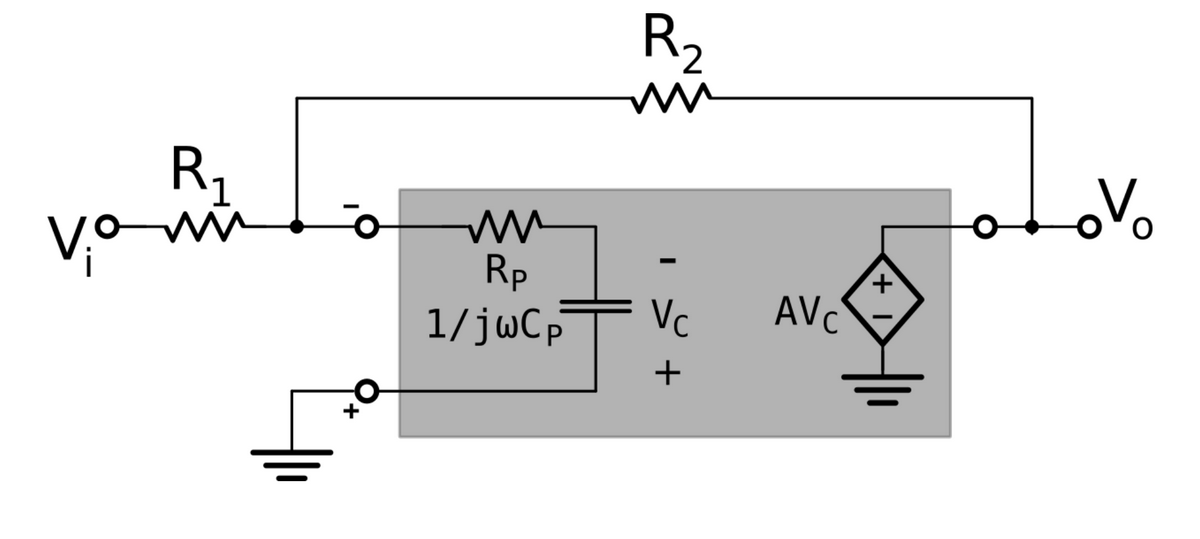
\includegraphics[width=1\columnwidth]{images/circuito.png}
    \caption{Circuito com amp op em configuração inversora.}
\end{figure}


\newpage
\subsection{Análise simbólica}


Podemos realizar a análise do circuito utilizando análise nodal.


\begin{equation}
    \begin{aligned}
        0       & = \frac{V_{a}}{R_{p} + \frac{1}{C_{p} j w}} + \frac{V_{a} - V_{o}}{R_{2}} + \frac{V_{a} - V_{i}}{R_{1}} \\
        - V_{c} & = \frac{V_{a}}{C_{p} j w \left(R_{p} + \frac{1}{C_{p} j w}\right)}                                      \\
        V_{o}   & = A V_{c}
    \end{aligned}
\end{equation}


Resolvendo as equações para $V_o$ obtemos que $V_o$ é dado por:


\begin{equation}
    - \frac{A R_{2} V_{i}}{A R_{1} + C_{p} R_{1} R_{2} j w + C_{p} R_{1} R_{p} j w + C_{p} R_{2} R_{p} j w
        + R_{1} + R_{2}}
\end{equation}


Aqui fazemos a seguinte simplificação $R_p >> R_1$ , $R_p >> R_2$, e $A >> 1$:


\begin{equation}
    V_o = - \frac{A R_{2} V_{i}}{A R_{1} + C_{p} R_{p} j w \left(R_{1} + R_{2}\right)}
\end{equation}


Com esta simplificação fazemos $\frac{V_o}{V_i}$ para obter a função transferência $H\left(jw\right)$:


\begin{equation}
    H\left(jw\right) = - \frac{A R_{2}}{A R_{1} + C_{p} R_{p} j w \left(R_{1} + R_{2}\right)}
\end{equation}


Agora podemos reorganiza-la no formato de um filtro passa-baixa para achar o ganho $K$, e a frequência de corte $w_c$:


\begin{equation}
    \begin{aligned}
        H(jw) & = - \frac{K w_c}{jw + w_c} \\
        w_p   & = \frac{1}{R_p C_p}        \\
        K     & = \frac{R_2}{R_1}          \\
        w_c   & = \frac{A w_p}{1 + K}
    \end{aligned}
\end{equation}


Podemos também achar o valor absoluto de $H(jw)$:


\begin{equation}
    \lvert H(jw) \rvert = \frac{\left|{K w_{c}}\right|}{\sqrt{w^{2} + w_{c}^{2}}}
\end{equation}


\subsection{Análise numérica}


Aqui utilizaremos as equações (5) e (6) para implementar o circuito discutido acima com dois conjuntos de valores, os conjuntos diferem apenas em seu $R_2$


Para ambos circuitos utilizaremos os seguintes valores:


\begin{equation}
    \begin{aligned}
        R_1 & = 4.7k \varOmega \\
        w_p & = 2 \pi 1k rad/s \\
        A   & = 10^5
    \end{aligned}
\end{equation}


\subsubsection{Circuito 1}


Neste utilizaremos o valor  $R_2 = 22k$:


Isto nos dá:


\begin{equation}
    \begin{aligned}
        K   & = 4.68                     \\
        w_c & = 1.10 \times 10^{6} rad/s
    \end{aligned}
\end{equation}


\begin{center}
    \begin{tabular}{ |c|c|c| }
        \hline
        freq rad/s & freq Hz         & $\lvert H(jw) \rvert$ \\
        $0.5 w_c$  & $88014.98 Hz$   & 4.19                  \\
        $w_c$      & $176029.96 Hz$  & 3.31                  \\
        $2 w_c$    & $352059.93 Hz$  & 2.09                  \\
        $4 w_c$    & $704119.85 Hz$  & 1.14                  \\
        $10 w_c$   & $1760299.63 Hz$ & 0.47                  \\
        $20 w_c$   & $3520599.25 Hz$ & 0.23                  \\
        $40 w_c$   & $7041198.50 Hz$ & 0.12                  \\
        \hline
    \end{tabular}
\end{center}


\subsubsection{Circuito 2}


Neste utilizaremos o valor  $R_2 = 560k$:


Isto nos dá:


\begin{equation}
    \begin{aligned}
        K   & = 119.15      \\
        w_c & = 52295 rad/s
    \end{aligned}
\end{equation}


\begin{center}
    \begin{tabular}{ |c|c|c| }
        \hline
        freq rad/s & freq Hz      & $\lvert H(jw) \rvert$ \\
        $0.5 w_c$  & $4161.50 Hz$ & 106.57                \\
        $w_c$      & $8323 Hz$    & 84.25                 \\
        $5 w_c$    & $41615 Hz$   & 23.37                 \\
        $20 w_c$   & $166460 Hz$  & 5.95                  \\
        $50 w_c$   & $416150 Hz$  & 2.38                  \\
        $200 w_c$  & $1664600 Hz$ & 0.60                  \\
        $500 w_c$  & $4161501 Hz$ & 0.24                  \\
        $1000 w_c$ & $8323003 Hz$ & 0.12                  \\
        \hline
    \end{tabular}
\end{center}


\newpage


\subsubsection{Gráfico dos exemplos}


\begin{figure}[h]
    \centering
    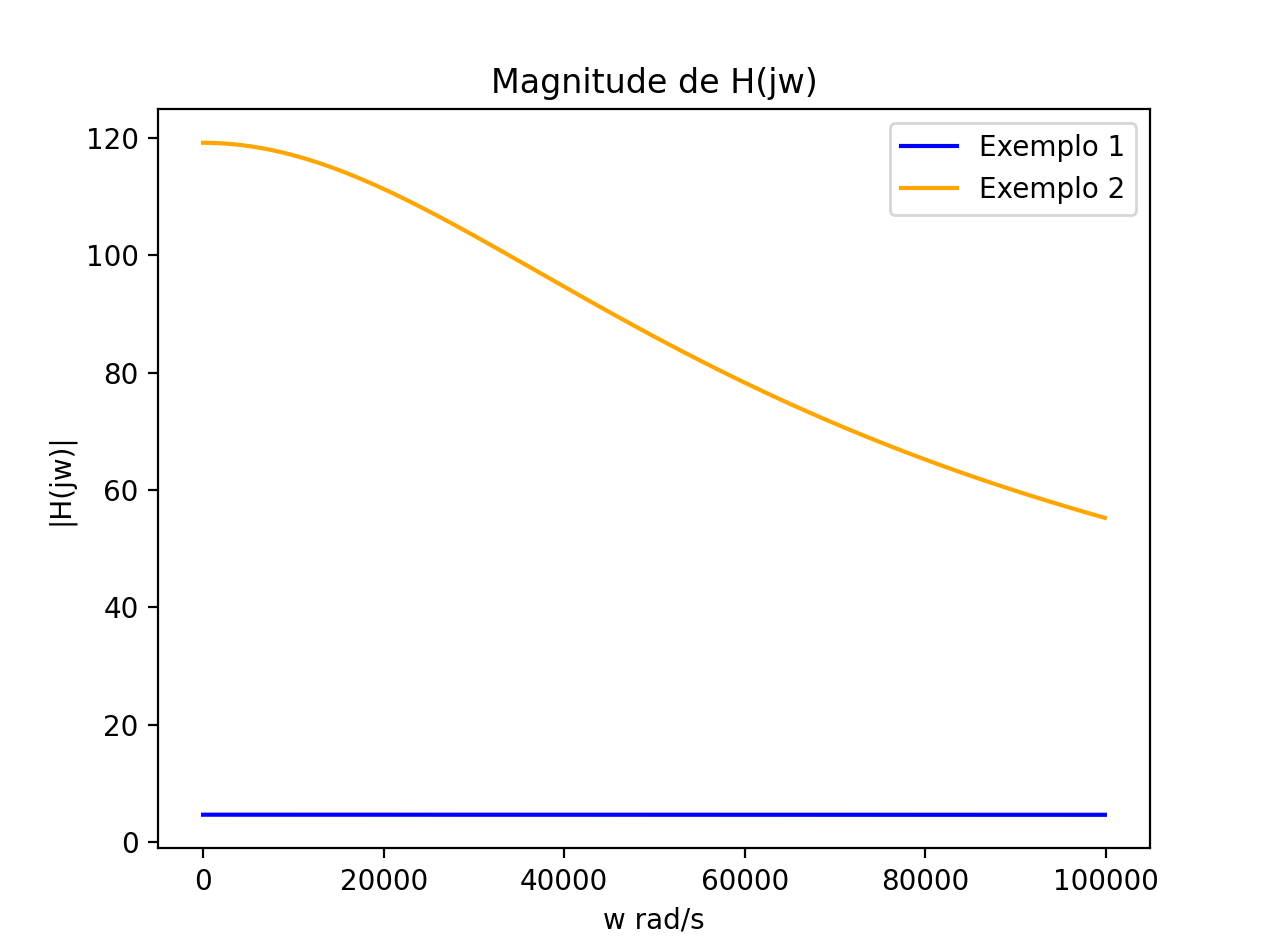
\includegraphics[width=1\columnwidth]{images/plot_bode.png}
    \caption{Gráfico da magnitude pela frequência dos exemplos 1 e 2.}
\end{figure}


\newpage


\section{Medições em laboratório}


Montaremos os dois circuitos discutidos acima em laboratório, e mediremos a tensão de entrada e saída para várias frequências, e com isto obteremos a magnitude da função transferência para frequências diversas.


\begin{figure}[h]
    \centering
    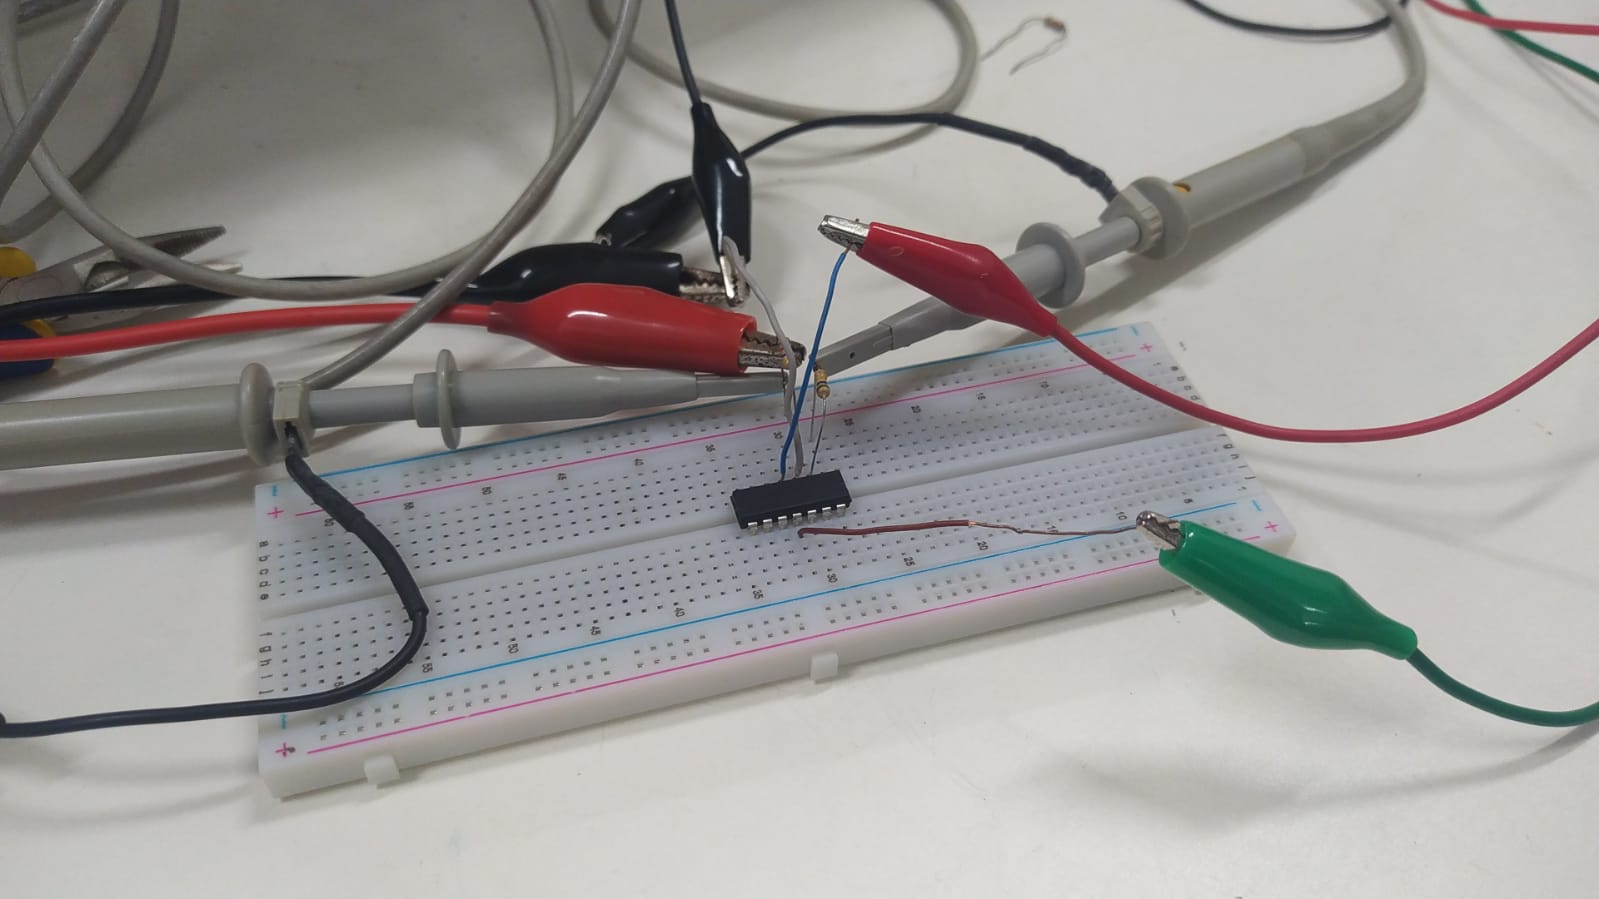
\includegraphics[width=1\columnwidth]{images/circuitoreal.jpeg}
    \caption{Foto do circuito montado em laboratório.}
\end{figure}


\subsection{Circuito 1}


\subsubsection{Valores dos componentes}


\begin{equation}
    \begin{aligned}
        R_1 = 4.65k \varOmega \\
        R_2 = 21.9k \varOmega \\
    \end{aligned}
\end{equation}


\subsubsection{Frequência de corte}


Identificamos a frequência de corte como sendo $f_c = 210 kHz$.


\subsubsection{Valores medidos}


\begin{figure}[H]
    \centering
    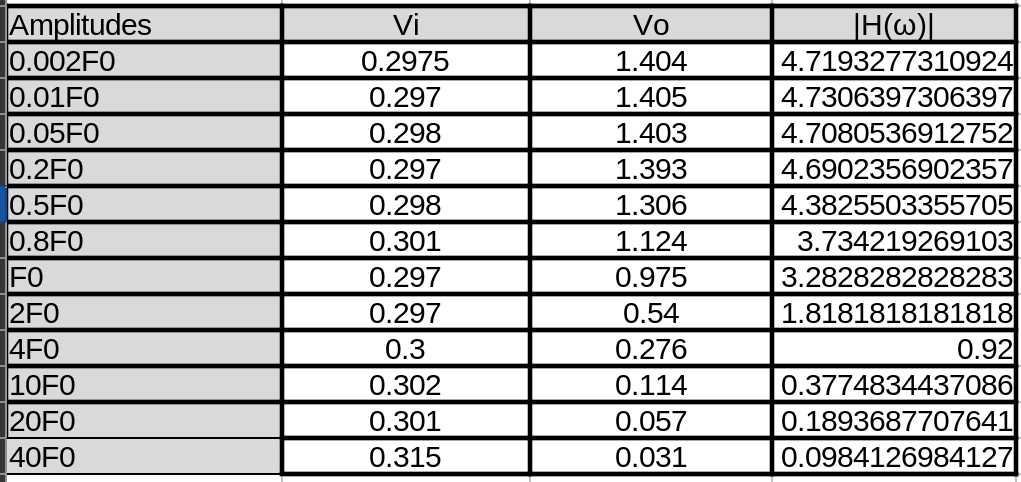
\includegraphics[width=1\columnwidth]{images/valores1.png}
    \caption{Tabela de magnitude para uma gama de valores de frequência.}
\end{figure}


\subsubsection{Fotos do osciloscópio}


\begin{figure}[H]
    \centering
    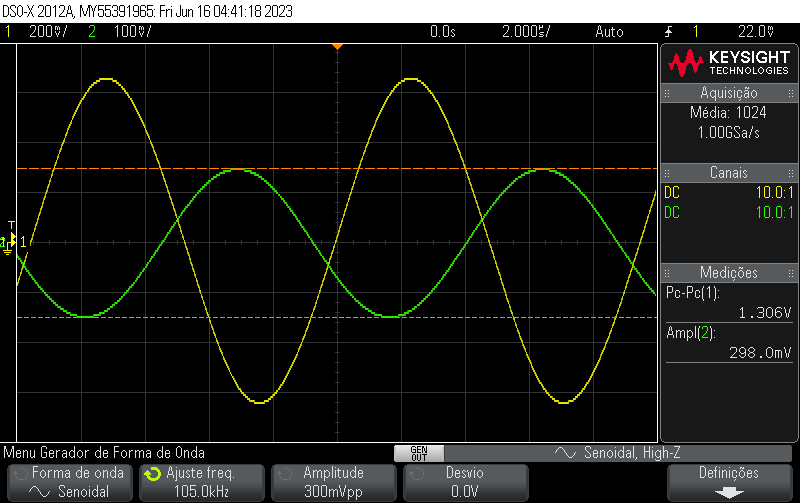
\includegraphics[width=1\columnwidth]{images/exemplo1_meio_fc.png}
    \caption{Imagem da onda no osciloscópio para 0.5 $f_c$.}
\end{figure}


\begin{figure}[H]
    \centering
    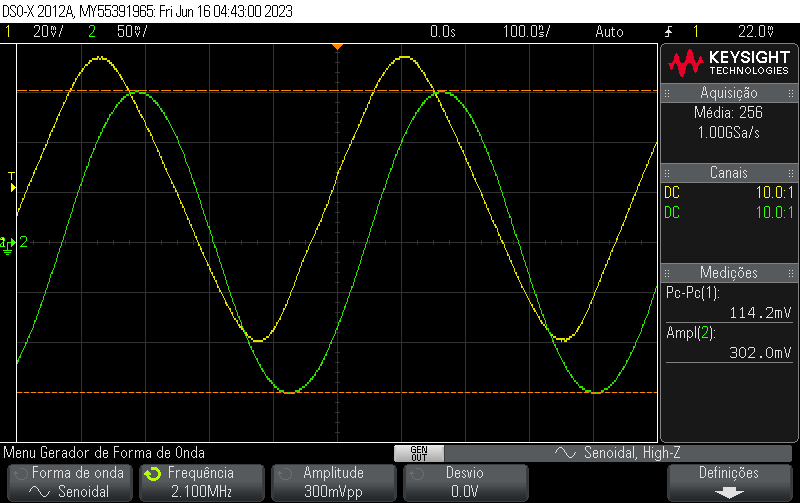
\includegraphics[width=1\columnwidth]{images/exemplo1_10_fc.png}
    \caption{Imagem da onda no osciloscópio para 10 $f_c$.}
\end{figure}


\begin{figure}[H]
    \centering
    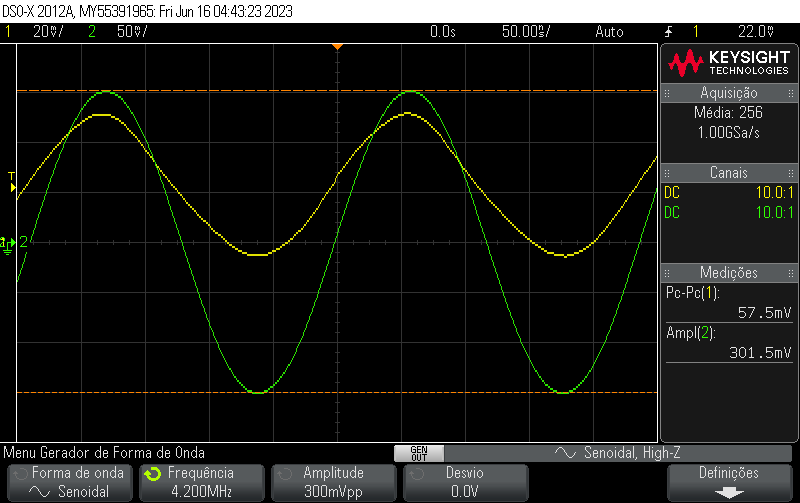
\includegraphics[width=1\columnwidth]{images/exemplo1_20_fc.png}
    \caption{Imagem da onda no osciloscópio para 20 $f_c$.}
\end{figure}
\newpage


\subsection{Circuito 2}


\subsubsection{Valores dos componentes}


\begin{equation}
    \begin{aligned}
        R_1 = 4.65k \varOmega \\
        R_2 = 550k \varOmega  \\
    \end{aligned}
\end{equation}


\subsubsection{Frequência de corte}


Identificamos a frequência de corte como sendo $f_c = 11800 kHz$.


\subsubsection{Valores medidos}


\begin{figure}[h]
    \centering
    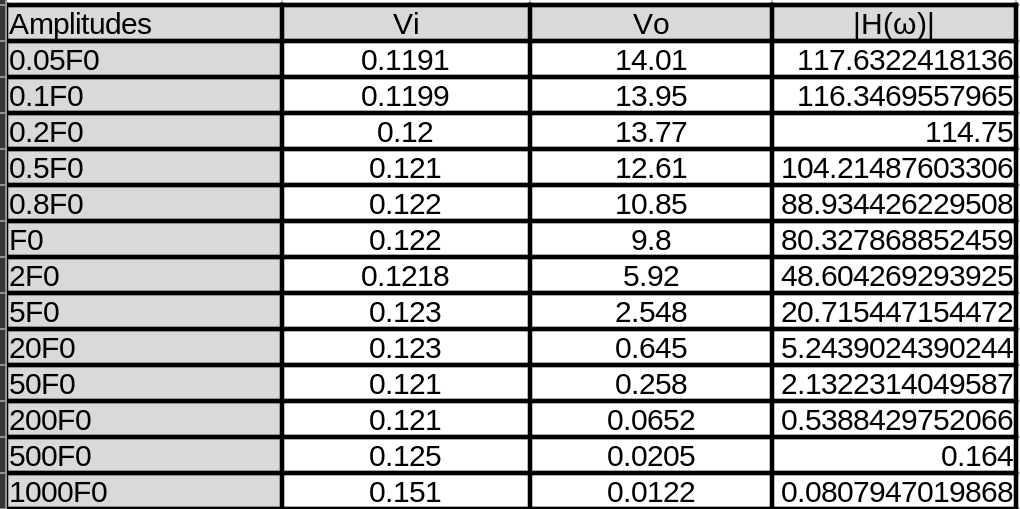
\includegraphics[width=1\columnwidth]{images/valores2.png}
    \caption{Tabela de magnitude para uma gama de valores de frequência.}
\end{figure}


\subsubsection{Fotos do osciloscópio}


\begin{figure}[h]
    \centering
    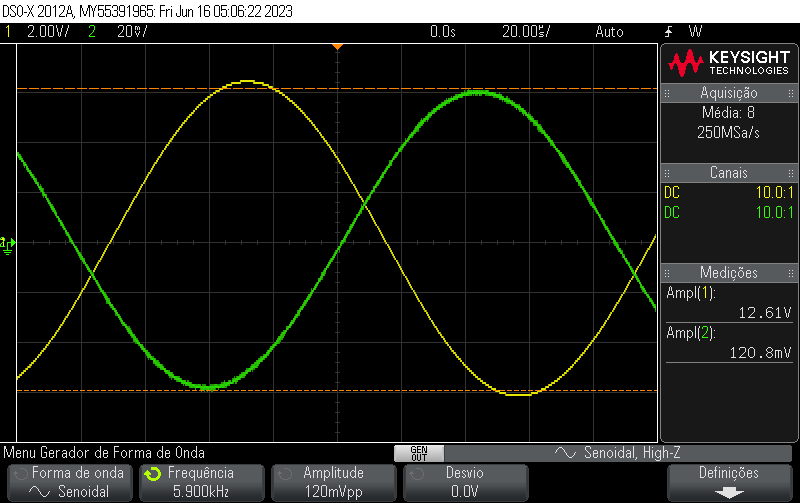
\includegraphics[width=1\columnwidth]{images/exemplo2_meio_fc.png}
    \caption{Imagem da onda no osciloscópio para 0.5 $f_c$.}
\end{figure}


\begin{figure}[h]
    \centering
    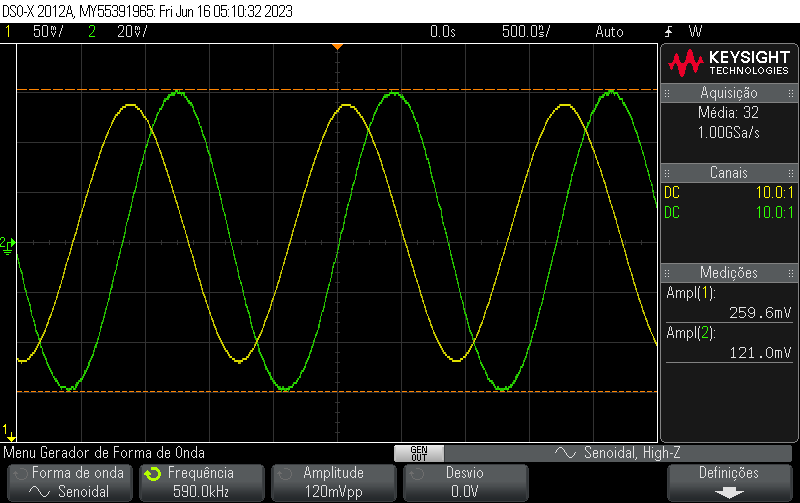
\includegraphics[width=1\columnwidth]{images/exemplo2_50_fc.png}
    \caption{Imagem da onda no osciloscópio para 50 $f_c$.}
\end{figure}


\begin{figure}[h]
    \centering
    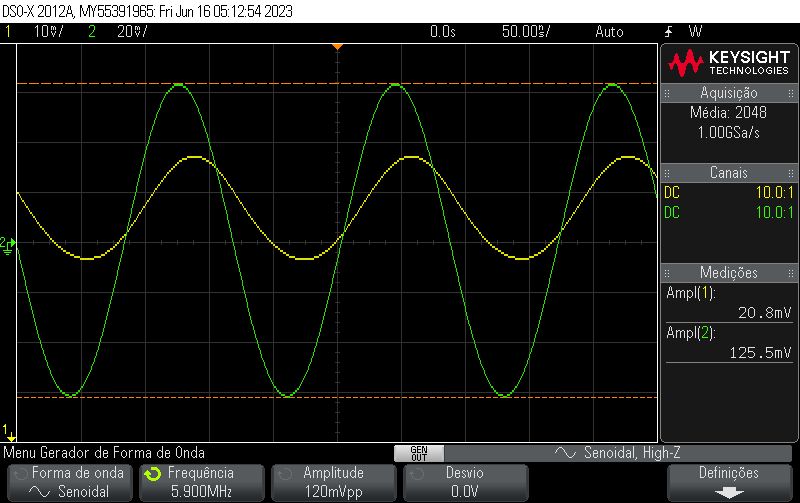
\includegraphics[width=1\columnwidth]{images/exemplo2_500_fc.png}
    \caption{Imagem da onda no osciloscópio para 500 $f_c$.}
\end{figure}


\newpage


\section{Análise dos resultados}


Obtivemos as magnitudes de $H(jw)$ dos exemplos nas figuras (3) e (6), as utilizarei no algoritmo de ajuste de curva que foi disponibilizado no Classroom.


\subsection{Circuito 1}


\subsubsection{Ajuste de curva}


Pelo código de ajuste de curva obtivemos os seguintes valores:


\begin{equation}
    \begin{aligned}
        K   & = -4.9                            \\
        f_c & = 168452.6 Hz = 1.06 * 10^6 rad/s
    \end{aligned}
\end{equation}


Que são coerentes e próximos com os valores achados anteriormente na equação (8).


\subsubsection{Gráfico de Bode}


\begin{figure}[H]
    \centering
    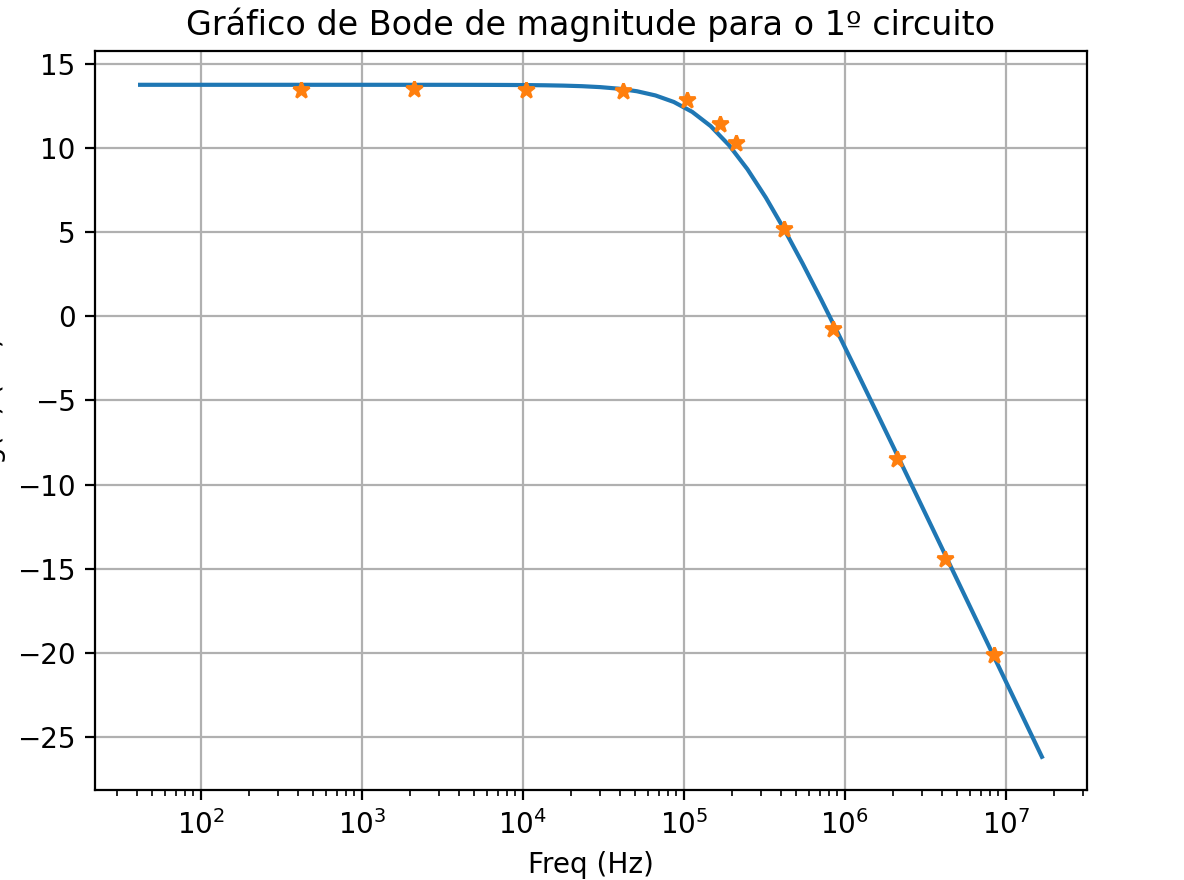
\includegraphics[width=1\columnwidth]{images/bode1.png}
    \caption{Gráfico de Bode para o primeiro circuito.}
\end{figure}


\subsection{Circuito 2}


\subsubsection{Ajuste de curva}


Pelo código de ajuste de curva obtivemos os seguintes valores:


\begin{equation}
    \begin{aligned}
        K   & = -120.1                   \\
        f_c & =  9701.2 Hz = 60954 rad/s
    \end{aligned}
\end{equation}


Que são coerentes e próximos com os valores achados anteriormente na equação (9).


\subsubsection{Gráfico de Bode}


\begin{figure}[H]
    \centering
    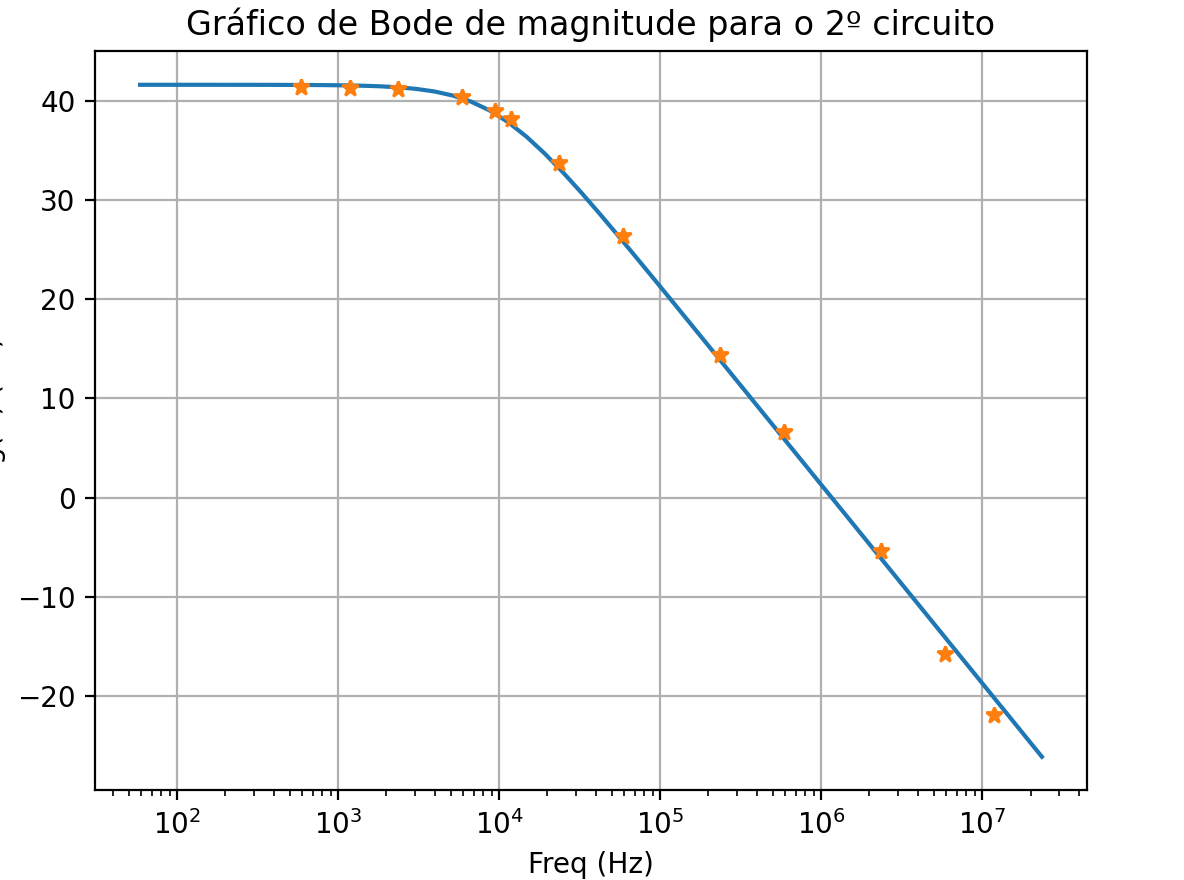
\includegraphics[width=1\columnwidth]{images/bode2.png}
    \caption{Gráfico de Bode para o segundo circuito.}
\end{figure}






\subsection{Gráfico de Bode de ambos circuitos.}


\begin{figure}[H]
    \centering
    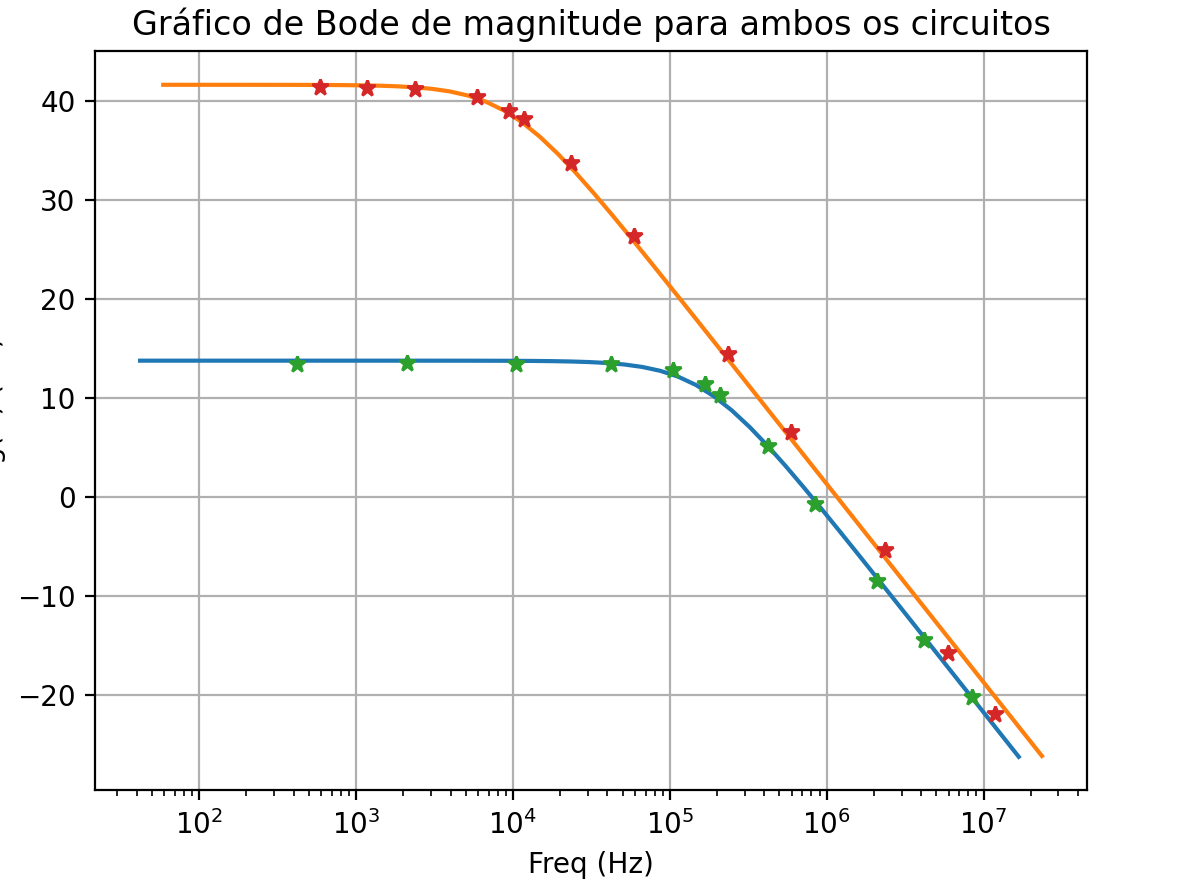
\includegraphics[width=1\columnwidth]{images/bodeboth.png}
    \caption{Gráfico de Bode para ambos circuitos sobrepostos.}
\end{figure}


\section{Conclusões}


Conseguimos com sucesso fazer a análise simbólica e numérica com a biblioteca sympy do Python, e comparamos os resultados com os obtidos experimentalmente.

Nos resultados práticos, obtivemos parâmetros $K$ e $w_c$ bastante similares aos obtidos numericamente.

Observamos que ambos circuitos se comportam como filtros passa-baixa inversores de primeira ordem, que era esperado devido a forma da equação que encontramos na análise preliminar.

Em suma creio que tivemos sucesso em nos familiarizar com as ferramentas de análise de circuitos eletrônicos, e métodos para análise numérica e simbólica.



\end{document}